%% The first command in your LaTeX source must be the \documentclass command.
\documentclass[10pt, sigconf]{acmart}

\settopmatter{printacmref=false, printccs=false, printfolios=true}

\usepackage{booktabs} % For formal tables
%\usepackage{cite}


\graphicspath{{figure/}{figures/}}

%% \BibTeX command to typeset BibTeX logo in the docs
\AtBeginDocument{%
  \providecommand\BibTeX{{%
    Bib\TeX}}}

% Copyright
%\setcopyright{none}
\setcopyright{acmcopyright}
%\setcopyright{acmlicensed}
% \setcopyright{rightsretained}
%\setcopyright{usgov}
%\setcopyright{usgovmixed}
%\setcopyright{cagov}
%\setcopyright{cagovmixed}

% DOI
\acmDOI{XXXXXXX.XXXXXXX}

% ISBN
\acmISBN{979-8-4007-1737-6}

%Conference
\acmConference[ICIT 2024]{2024 The 12th International Conference on Information Technology: IoT and Smart City}{December 13-15, 2024}{Kuala Lumpur}
\acmYear{2024}
\copyrightyear{2024}

\acmPrice{15.00}

\begin{document}
\title{Micro Leak Detection of Natural Gas for Residential Users Based on Gas Flowmeters}
%\titlenote{Produces the permission block, and copyright information}
%\subtitle{Paper \#, XXX pages}

\author{Alex Da Yin}
\orcid{0009-0001-0257-6500}
\authornotemark[1]
\affiliation{%
  \institution{Weeg Electronics Co,. LTD}
  \streetaddress{Building B1, South District, Hengshan Road}
  \city{Changzhou}
  \state{Jiangsu}
  \country{China}
  \postcode{213000 CN}
}
\email{d.yin@weegcn.cn}
\email{dyin1900@gmail.com}

\author{Weiping Ni}
\affiliation{%
  \institution{Weeg Electronics Co,. LTD}
  \city{Changzhou}
  \state{Jiangsu}
  \country{China}
}
\email{wp.ni@weegcn.cn}

\author{Fangcun Shu}
\affiliation{%
  \institution{Weeg Electronics Co,. LTD}
  \city{Changzhou}
  \state{Jiangsu}
  \country{China}
}
\email{fc.shu@weegcn.cn}


\renewcommand{\shortauthors}{Yin et al.}


\begin{abstract}
This paper presents a novel approach to detecting small residential gas leaks through a seq2seq generative model-based algorithm, termed the Weeg algorithm. Using real-world data from household membrane gas flowmeters and simulating both normal and leak conditions, we benchmarked the Weeg algorithm against traditional detection methods. The evaluation was performed on a dataset containing 86 leakage samples and 1103 non-leakage samples. The Weeg algorithm demonstrated significant improvements, achieving an accuracy of 90.2\% and an F1 score of 0.458, while reducing false positive rates by 92.8\% compared to conventional algorithms. Our approach eliminates the need for additional sensors, offering a cost-effective solution for residential gas leak detection.
\end{abstract}


%% The code below is generated by the tool at http://dl.acm.org/ccs.cfm.
%% Please copy and paste the code instead of the example below.
\begin{CCSXML}
<ccs2012>
   <concept>
       <concept_id>10003752.10010070.10010071.10010074</concept_id>
       <concept_desc>Theory of computation~Unsupervised learning and clustering</concept_desc>
       <concept_significance>500</concept_significance>
       </concept>
   <concept>
       <concept_id>10010520.10010553.10003238</concept_id>
       <concept_desc>Computer systems organization~Sensor networks</concept_desc>
       <concept_significance>300</concept_significance>
       </concept>
 </ccs2012>
\end{CCSXML}

\ccsdesc[500]{Theory of computation~Unsupervised learning and clustering}
\ccsdesc[300]{Computer systems organization~Sensor networks}
\ccsdesc{Theory of computation~Theory and algorithms for application domains}
\ccsdesc[100]{Information systems~Information systems applications}


\keywords{leakage detection, time series, IoT, natural gas, neural network}

%% A "teaser" image appears between the author and affiliation
%% information and the body of the document, and typically spans the
%% page.
%\begin{teaserfigure}
%  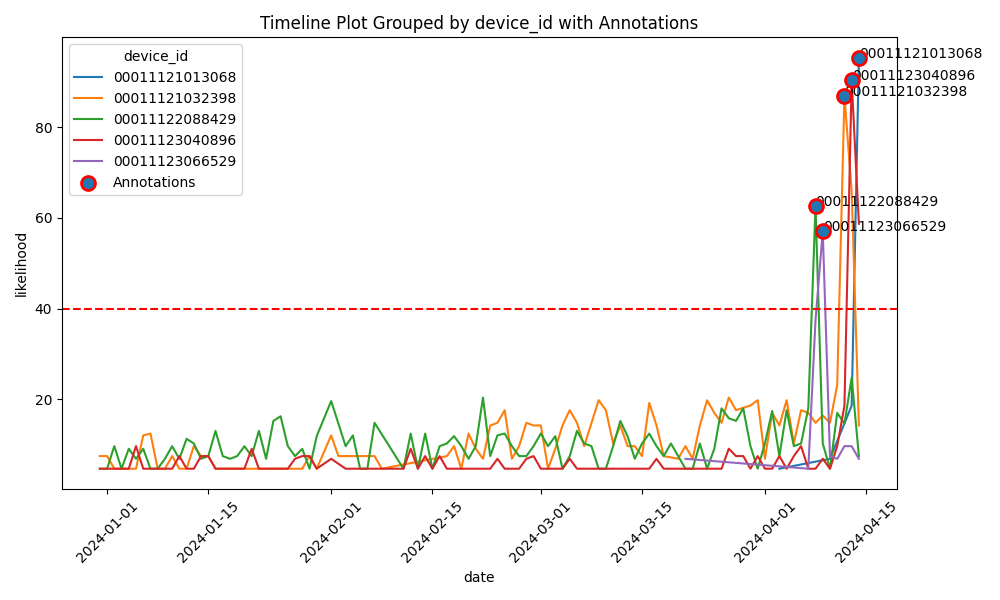
\includegraphics[width=\textwidth]{timeline}
%  \caption{Daily scoring curve for the likelihood of a small gas leak occurring at a residential client.}
%  \Description{The algorithm output is the probability that a microleak event has occurred, and the higher the score, the higher the probability of leakage.When the output of the algorithm exceeds the threshold, the system pushes alarm information to the management platform and users.}
%  \label{fig:timeline}
%\end{teaserfigure}

%%
%% This command processes the author and affiliation and title
%% information and builds the first part of the formatted document.
\maketitle

\section{Introduction}

The main object of urban gas supply is resident users and public building users, especially the former is very large, but the gas flow value of each household is very small, and it must be one household with (at least) one meter device \cite{fraiwan2011wireless, omidvarborna2021low}. As of 2024, the gas flowmeters used by residential users in China are generally membrane gas flowmeters.  With the growth of the demand for urban gas, the safety problem has become increasingly prominent. China Gas Association (CGA) statistics found that in various types of accidents, residential user accidents are the most frequent, only in the first half of 2021 there were 305, accounting fosr 56\% of the total \cite{zhang2023building}. In general, each household of residential users is an independent unit (apartment or villa), with a large user base and dispersed address distribution, and the scheme of "safety inspection by gas company one by one" lacks operability. 

At present, the Internet of Things (IoT) devices are mainly used to remotely monitor gas usage \cite{suma2019gas}, collect the flow data of residential users through the sensors of smart gas meters, and apply relevant algorithms to identify potential gas leakage events \cite{ali2022solution, li2023accurate}. The advantage of direct use of flow data for leakage event identification is obvious, the solution only needs to use existing flow metering equipment, and does not need to set up additional types of sensors (e.g., acoustic emission devices or gas concentration sensors) \cite{zaman2020review}.

Existing detection methods are generally good at identifying large scale breaches or leaks in simple systems, but are inadequate at detecting small leaks early on \cite{ge2008analysis, tian2016study, rahmat2017water}. For example, based on statistical experience, it can be assumed that the probability of a leak event and the size of a leak approximately follow a Gaussian distribution, from which it can be inferred that small leaks account for the majority of (detectable) residential gas leaks. However, based on historical reported data, traditional leak detection schemes rarely detect small leak events \cite{dange2024automated}. From this, it can be seen that traditional leak detection schemes underestimate the reporting of small leaks. Traditional schemes struggle to distinguish between normal gas usage patterns and abnormal conditions that could indicate a leak, and lack the sensitivity to identify small leaks \cite{salhi2019early, sekhavati2022computational, khan2020sensor}.

To address the above issue, we propose a small leakage detection scheme for residential gas based on membrane flowmeter. Firstly, we analyze the pulse metering mode of the membrane flowmeter, and establish the mathematical and physical model of the single source steady flow condition. Through the mathematical physical model, we can realize the transformation from the actual flow to the nominal flow (the final output pulse sequence of the flow metering equipment). We then designed a small data set containing small leakage events by referring to the hourly gas flow rates of several typical residential gas equipment, including 8000 serial pairs of actual and nominal flow rates (of which 4000 samples had persistent small leakage events). We use this synthetic data set to train a generative model of seq2seq based on the stable diffusion model for inverting the nominal flow to the actual flow. Using real data collected by the sensors from July to December 2023 as input, we used the generation model to unsupervised label real-world nominal flow for leakage events. Based on real data sets with unsupervised labeling, we trained a lightweight network to achieve approximate real-time detection of small leaks. In addition, we propose a confidence calculation method to quantify the user's risk of a small gas leak event over a continuous 24-hour period.

The organization of this paper is as follows: \textbf{Section 2} reviews related work on natural gas pipeline leak detection, providing background for the study. \textbf{Section 3} introduces the mathematical and physical model under single-source steady flow conditions, laying the foundation for understanding flow behavior. \textbf{Section 4} explains the creation of both the synthetic dataset and the unsupervised labeled dataset, detailing the data simulation process, the seq2seq generative model, and the unsupervised labeling method. In \textbf{Section 5}, we test the proposed methods using a manually labeled dataset to evaluate performance. Finally, \textbf{Section 6} concludes with a brief summary of the findings.

\section{Related Work}
\subsection{Traditional Gas Leak Detection Methods}
% Current sensor-based approaches

\subsection{Early Gas Leakage Detection for Home}
% Current home-specific content

\subsection{Machine Learning Approaches}
% Add content about ML/DL methods

\subsection{Low-Cost Air Quality and Gas Leak Detection}
% Current content

\section{Mathematical and Physical Model}

Gas flow meters are essential devices for accurately measuring the flow rate and volume of gases in industrial and residential settings. Various types of flow meters are used, each employing different principles to generate pulse signals corresponding to gas flow. These pulse signals can be analyzed to form time series data, which is crucial for monitoring and diagnosing gas usage patterns and system health. Below is a detailed explanation of the pulse time series generation process for two common types of gas flow meters: membrane flow meters and turbine flow meters, along with the mathematical models governing their operation.

\subsection{Membrane Flow Meter}

The membrane (or diaphragm) flow meter operates by periodically filling a chamber with gas and then discharging it, converting the cyclic filling process into pulse signals. It is commonly used in residential and commercial gas metering due to its reliability under varying pressure conditions.

The membrane flow meter generates a pulse when a fixed volume of gas, $V$ (in m³), fills the chamber. The gas flow rate into the chamber is described as a time-varying function $f(t)$ (in m³/s). The time required to fill the chamber, $T$, is calculated by integrating the flow rate over time until the total volume equals $V$:
\begin{equation}
   V = \int_{0}^{T} f(t) \, dt
\end{equation}

A pulse is generated every time the chamber fills completely. Over a given period $t$, the total number of pulses $N(t)$ can be calculated by dividing the total volume of gas that has passed through the meter by the chamber volume $V$:
\begin{equation}
   N(t) = \frac{1}{V} \int_{0}^{t} f(t') \, dt'
\end{equation}

\subsection{Turbine Flow Meter}

The turbine flow meter generates pulses based on the rotational speed of a turbine placed in the gas flow. The gas flow causes the turbine blades to rotate, and each rotation is converted into a pulse signal. The frequency of these pulses is directly proportional to the gas flow rate. This type of flow meter is widely used in industrial applications due to its precision and ability to measure large flow rates.

In a turbine flow meter, pulses are generated based on the accumulated rotation angle. Let $\Theta$ represent the threshold angle (in radians or degrees) after which a pulse is generated. The turbine’s rotational speed $\omega(t)$ (in radians per second) is related to the flow velocity $v(t)$. For small flow rates, the rotational speed is proportional to the flow velocity:
\begin{equation}
   \omega(t) = k \cdot v(t)
\end{equation}
where $k$ is a proportional constant.

A pulse is generated every time the accumulated angle reaches $\Theta$. The total number of pulses over time $t$, denoted as $N(t)$, can be calculated by integrating the rotational speed $\omega(t)$ over time and dividing by $\Theta$:
\begin{equation}
N(t) = \frac{1}{\Theta} \int_{0}^{t} \omega(t') \, dt'
\end{equation}

Alternatively, if the flow velocity $v(t)$ is known, we can express the pulse count in terms of the flow velocity:
\begin{equation}
   N(t) = \frac{k}{\Theta} \int_{0}^{t} v(t') \, dt'
\end{equation}

In both types of flow meters, the pulses generated over time form a time series, where each pulse corresponds to a discrete volume of gas passing through the meter. The time intervals between pulses provide insights into the flow rate, and any irregularities in these intervals could indicate system malfunctions, leaks, or abnormal usage patterns.

\section{Data Set Construction}

In this section, we outline the construction of the dataset used to train and evaluate our proposed leakage detection model. The dataset comprises both simulated data and real-world data. The key steps involved include data simulation, leveraging a seq2seq generative model for nominal-to-actual flow conversion, and unsupervised labeling of real-world data.

\subsection{Data Simulation}

The data simulation process is crucial for creating a controlled environment to study gas leakage events, especially when real-world leakage data is scarce or difficult to obtain. To address this, we generated a synthetic dataset by simulating gas consumption in residential settings, incorporating both normal usage and small leakage scenarios.

To replicate realistic gas flow patterns, we referred to the typical gas usage of common household appliances, such as water heaters, stoves, and boilers, as outlined in Table~\ref{tab:gas_consumption}. The simulation model was built on pulse metering principles derived from the operational characteristics of membrane gas flowmeters, mapping each device's gas consumption to nominal and actual flow rates under steady-state conditions. In China, the normal pressure for low-pressure natural gas used in residential applications ranges from 1.5 kPa to 3.0 kPa.

\begin{table}[htbp]  % "h" for here, "t" for top, "b" for bottom, "p" for page
  \caption{Typical Gas Equipment and Leakage Characteristics at Low Pressure (1.5-3.0 kPa)}
  \label{tab:gas_consumption}
  \begin{tabular}{cc}
    \toprule
    Equipment/Leakage & Gas Consumption (m³/hour) \\
    \midrule
    Gas Stove         & 0.2 - 0.3                 \\
    Gas Water Heater  & 1.2 - 1.5                 \\
    Gas Furnace       & 1.2 - 3.0                 \\
    Gas Dryer         & 0.6 - 0.75                \\
    Gas Micro-Leak    & 0.01 - 0.3               \\
    \bottomrule
  \end{tabular}
\end{table}

In a membrane flowmeter, the time between pulses varies according to the flow rate—longer at low flow rates and shorter at higher rates. To model multiple simultaneous gas usage events, we adjusted the flow calculations to account for the combined effects of various events. Figure~\ref{fig:actual_flow} illustrates a time series of actual flow rates, which includes the following event types:

\begin{itemize}
  \item \textbf{Simulated microleak}: Active throughout the entire period at a base rate of 0.05 m³/hour.
  \item \textbf{Simulated gas stove}: Activated during the interval [3/5, 4/5] of the total duration, with a base rate of 0.2 m³/hour.
  \item \textbf{Simulated timed water heater}: Triggered in each 1/6 cycle of the duration, active during the first 20\% of each cycle, starting at half the cycle length, with a base rate of 1.2 m³/hour.
\end{itemize}

Assuming the chamber capacity of the membrane gas flowmeter is 0.01 m³, we applied our mathematical model to convert the actual flow rates into nominal flow values, represented as pulse counts per minute. Figure~\ref{fig:nominal_flow} depicts this conversion. The comparison between actual and nominal flow rates is shown in Figure~\ref{fig:actual_vs_nominal}, highlighting the difference between the observed nominal flow (red line), the smoothed flow (blue line, via Gaussian filtering), and the actual flow (green line). As seen, neither the raw nominal flow nor the smoothed version accurately captures the true gas usage.

\begin{figure}[htbp]  % "h" for here, "t" for top, "b" for bottom, "p" for page
  \centering
  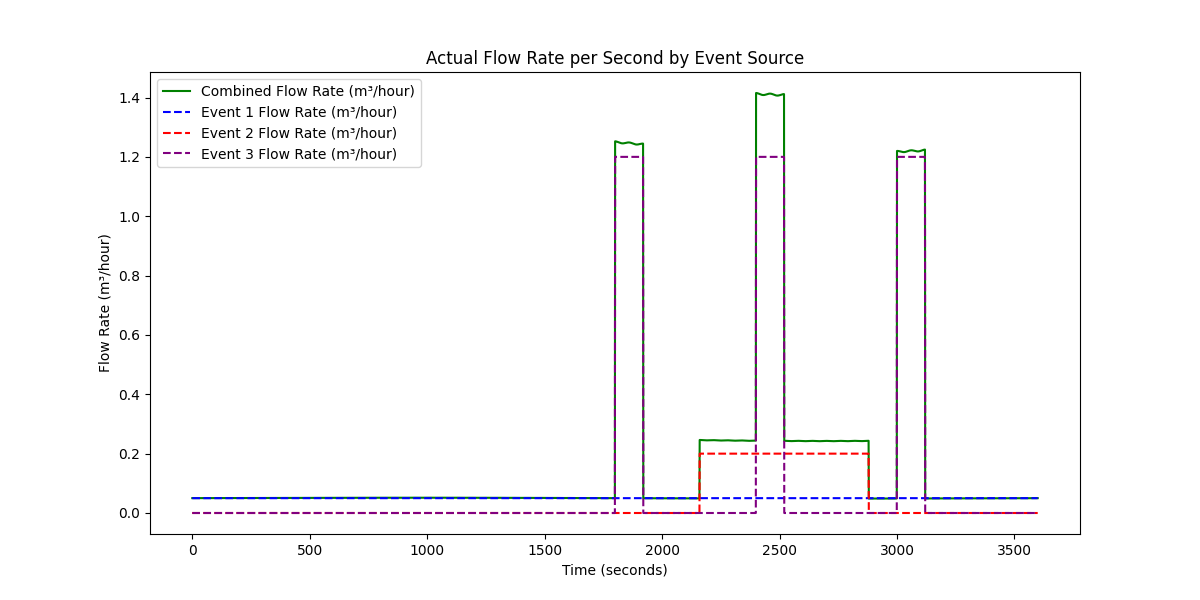
\includegraphics[width=\columnwidth]{actual_flow}
  \caption{Actual Flow Rate per Second by Event Source}
  \Description{
Event 1: Simulated microleak, active for the entire period at a rate of 0.05 m³/hour.
Event 2: Simulated gas stove, active during [3/5, 4/5] of the duration at 0.2 m³/hour.
Event 3: Simulated timed water heater, active during the first 20\% of every 1/6 cycle, starting at half the duration, at 1.2 m³/hour.}
  \label{fig:actual_flow}
\end{figure}

\begin{figure}[htbp]  % "h" for here, "t" for top, "b" for bottom, "p" for page
  \centering
  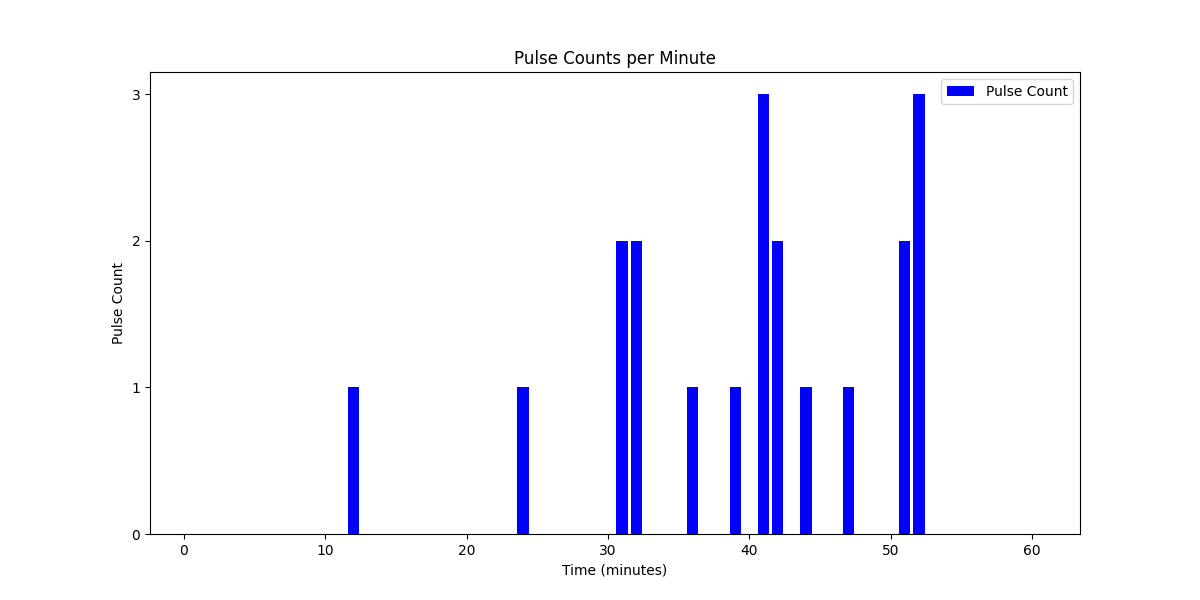
\includegraphics[width=\linewidth]{nominal_flow}
  \caption{Pulse Counts per Minute}
  \Description{The time series of pulse counts per minute from the gas flowmeter.}
  \label{fig:nominal_flow}
\end{figure}

\begin{figure}[htbp]
  \centering
  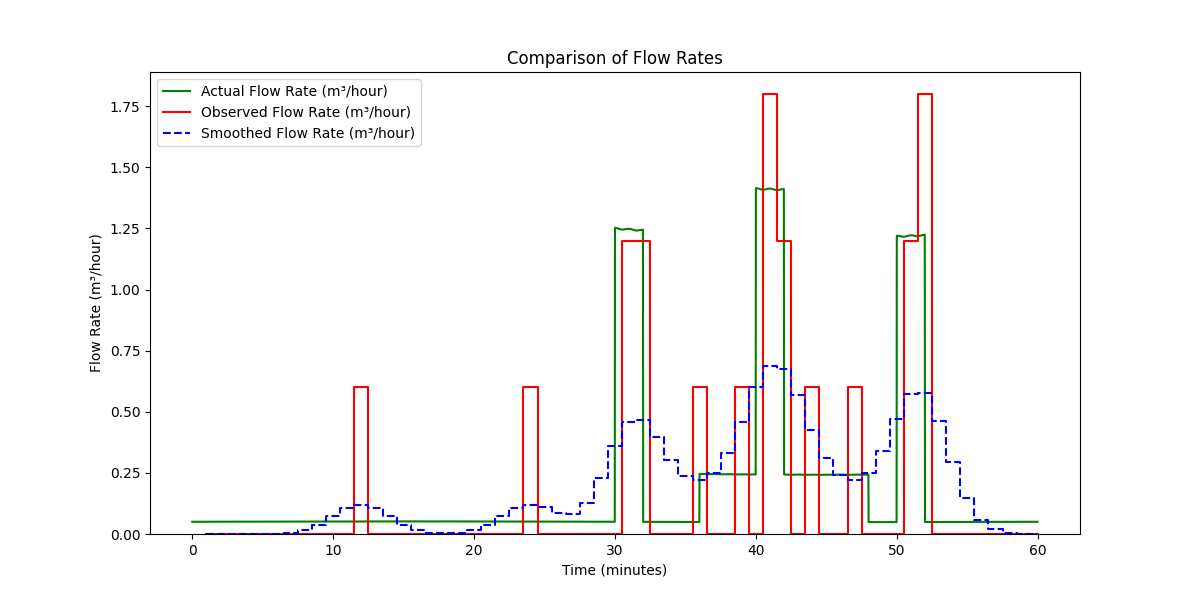
\includegraphics[width=\columnwidth]{actual_vs_nominal}
  \caption{Comparison of Actual vs Nominal Flow Rates. The red line shows the raw nominal flow readings from the flowmeter, the blue line represents the smoothed flow using Gaussian filtering (σ = 5), and the green line indicates the actual gas flow rate. Note the significant discrepancy between nominal and actual flow rates during low-flow periods.}
  \label{fig:actual_vs_nominal}
\end{figure}

The final dataset consists of 8000 time series samples, each representing an hourly gas flow rate. Of these, 4000 samples included simulated persistent small leakage events, designed to mimic real-world leak scenarios. Each simulated event was carefully calibrated to reflect the subtle deviations between nominal and actual flow rates that typically characterize small gas leaks. This simulation process provided a robust dataset for training and testing the generative model discussed in the next subsection.

\subsection{Seq2Seq Generative Model}

A critical aspect of our approach is the use of a seq2seq generative model to invert the nominal flow rates recorded by membrane flowmeters back to actual flow rates. This inversion is necessary because gas flowmeters primarily capture nominal values, while small leaks result in subtle deviations that are not directly measured.

We developed a seq2seq model based on the stable diffusion model, which has proven effective in capturing time-series variations. The model was trained using the simulated data set, with actual flow rates serving as the target and nominal flow rates as the input sequences. By learning the mapping between these two, the model can infer the true flow behavior under small leakage conditions.

The seq2seq architecture enabled us to generate continuous sequences of actual flow rates from nominal flow data, accounting for both normal usage and leakage patterns. This process is crucial for later stages, where real-world nominal flow data will be input into the trained model to estimate potential leakages. The generative model plays a pivotal role in unsupervised labeling, as discussed in the following section.

\subsection{Unsupervised Label}

Unsupervised labeling allows us to automatically detect potential small leakage events in real-world gas flow data without manual annotation. After training the seq2seq generative model on the synthetic dataset, we applied it to real sensor data collected from July to December 2023.

The generative model outputs estimations of actual flow rates from the nominal flow data recorded by membrane gas flowmeters. Any significant deviation between the estimated actual flow and the recorded nominal flow is flagged as a potential leakage event. By analyzing continuous flow data over extended periods, we can effectively label sections of the dataset where small leaks are likely occurring.

This method of unsupervised labeling is particularly advantageous because it eliminates the need for labor-intensive manual labeling of leakage events, which are often rare and difficult to observe directly. Additionally, it enables the generation of large labeled datasets from real-world data, facilitating the training of downstream models for real-time leak detection. 

\section{Experimental Results and Analysis}

In this section, we present the experimental results based on the residential gas leakage detection test dataset (20240101-20240414). The dataset contains 86 leakage samples and 1103 non-leakage samples. A detailed comparison of the performance of the traditional algorithm and the proposed Weeg algorithm under different alert thresholds is shown in Tables~\ref{tab:confusion_matrix} and ~\ref{tab:score_matrix}. The Weeg algorithm, with an alert threshold of 60, achieves the highest accuracy of 90.2\% and an F1 score of 0.458, outperforming the traditional method.

Table~\ref{tab:confusion_matrix} shows the confusion matrices for the traditional algorithm and the Weeg algorithm under two different alert thresholds (40 and 60). It is evident that the Weeg algorithm with a threshold of 60 provides the best balance between true positives (TP) and false positives (FP).

\begin{table*}[htbp]  % "h" for here, "t" for top, "b" for bottom, "p" for page
  \centering
  \caption{Confusion Matrix for Different Algorithms on the Test Dataset}
  \label{tab:confusion_matrix}
  \begin{tabular}{lcccc}
    \toprule
    Algorithm Model            & True Negatives (TN) & False Positives (FP) & False Negatives (FN) & True Positives (TP) \\
    \midrule
    Traditional Algorithm      & 0                   & 1103                 & 0                    & 86                  \\
    Weeg Algorithm (Threshold 40) & 815                 & 288                  & 18                   & 68                  \\
    Weeg Algorithm (Threshold 60) & 1024                & 79                   & 37                   & 49                  \\
    \bottomrule
  \end{tabular}
\end{table*}

Table~\ref{tab:score_matrix} summarizes the performance metrics, including accuracy, precision, recall, and F1 score, for the traditional algorithm and the Weeg algorithm. The Weeg algorithm with a threshold of 60 provides the highest accuracy of 90.2\%, a precision of 0.383, and an F1 score of 0.458. Although the recall of the traditional algorithm is 100\%, it achieves the lowest accuracy and F1 score due to a high rate of false positives.

\begin{table*}[htbp]
  \centering
  \caption{Performance Metrics for Different Algorithms on the Test Dataset (January-April 2024). Higher values are better for all metrics except False Positives (FP).}
  \label{tab:score_matrix}
  \begin{tabular}{lcccc}
    \toprule
    Algorithm Model            & Accuracy & Precision & Recall & F1 Score \\
    \midrule
    Traditional Algorithm      & 0.072    & 0.072     & \textbf{1.0}    & 0.135    \\
    Weeg Algorithm (Threshold 40) & 0.743    & 0.191     & 0.791   & 0.308    \\
    Weeg Algorithm (Threshold 60) & \textbf{0.902} & \textbf{0.383} & 0.570   & \textbf{0.458} \\
    \bottomrule
  \end{tabular}
\end{table*}

Figures~\ref{fig:traditional_model} and \ref{fig:vig_60_model} visualize the results of the traditional algorithm and the Weeg algorithm for alert thresholds 60. Dark points in the figures indicate incorrect predictions. The Weeg algorithm (Threshold 60) has the fewest errors compared to other methods.

\begin{figure}[htbp]  % "h" for here, "t" for top, "b" for bottom, "p" for page
  \centering
  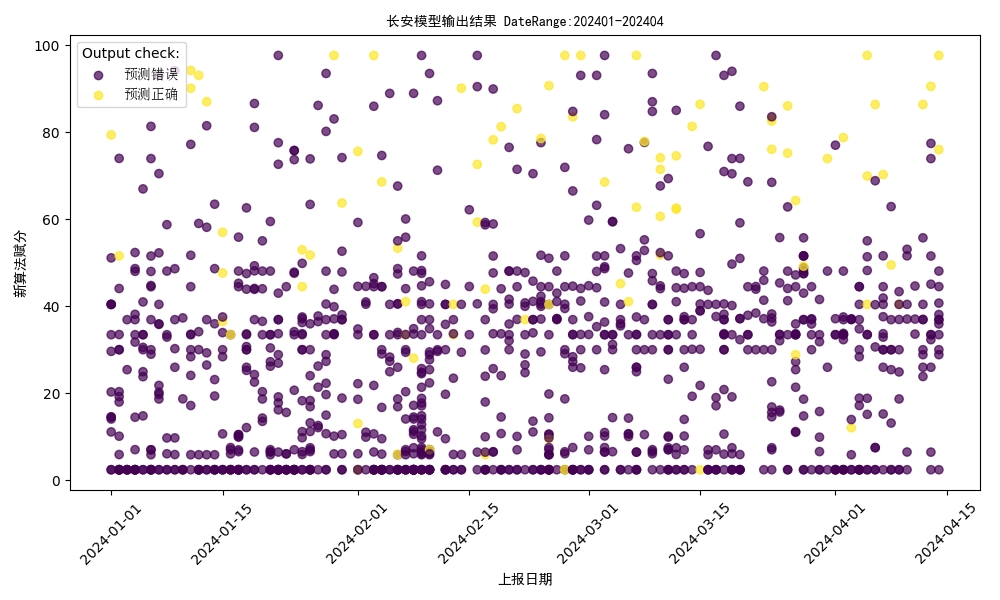
\includegraphics[width=0.8\linewidth]{ResultsForOldModel.png}
  \caption{Results of the Traditional Algorithm}
  \label{fig:traditional_model}
\end{figure}

\begin{figure}[htbp]  % "h" for here, "t" for top, "b" for bottom, "p" for page
  \centering
  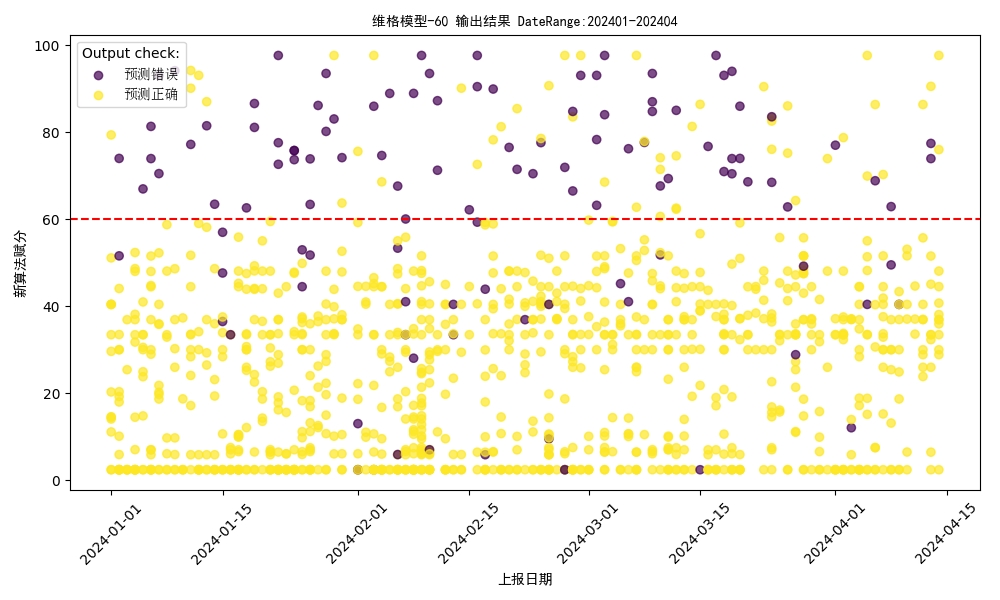
\includegraphics[width=0.8\linewidth]{ResultsForNewModel-60.png}
  \caption{Results of the Weeg Algorithm (Threshold 60)}
  \label{fig:vig_60_model}
\end{figure}

\section{Conclusions}

In this study, we presented a novel leakage detection algorithm (Weeg algorithm) and evaluated its performance against traditional algorithms using real-world residential gas usage data. Our approach demonstrates significant improvements in accuracy and overall detection performance, particularly when using a threshold of 60 for the alert system.

The results show that the Weeg algorithm achieves an accuracy of 90.2\%, with an F1 score of 0.458, significantly outperforming the traditional algorithm, which yielded an accuracy of only 7.2\% and an F1 score of 0.135. The improvement in precision, especially at higher thresholds, indicates that the proposed method reduces false positives while maintaining a balanced recall.

Furthermore, the visualizations of the detection results confirm that the Weeg algorithm successfully mitigates the errors present in the traditional method, offering a more reliable and efficient solution for early leakage detection.

The proposed Weeg algorithm represents a substantial step forward in the field of residential gas leakage detection. Future work will focus on further refining the algorithm to improve precision and adaptability across different environmental and operational conditions, as well as scaling its application to larger urban gas networks.

\begin{acks}
This work was supported by Chang'an Natural Gas Co., LTD in Xi'an, China. We are very grateful to Hangxing Hao for his support on the experiment and the feedback on our algorithm.
\end{acks}

\bibliographystyle{ACM-Reference-Format}
\bibliography{references}

%\appendix

\end{document}
\endinput
